%\begin{itemize}
%\item so we had a focus group to actually elaborate the aprroach
%\item then we used explorative prototyping to elicit the initial version of the prototype and then refined that by means of case study, we could mention that we used ATC as an action-research source (this is what we are doing now internally in WP2 actually)
%\item ...
%\end{itemize}
%
%The work we elaborated in this paper is stemming from the following research question:
%
%\begin{center}
%\emph{``What are the sub-optimal structural"}
%\end{center}
%% \comment{I would say if we connect it to the special need in DICE would makes more sense?}
%
%This research question emerged as part of our work within the DICE EU H2020 project~\cite{dice2020}
%%\footnote{\url{http://www.dice-h2020.eu/}} 
%where we evaluated our case-study owners' scenarios and found that their continuous architecting needs were: (a) focusing on the topological abstractions and surrounding architectural specifications; (b) focusing on bridging the gap between insights from Ops to (re-)work at the Dev level; (c) their needs primarily consisted in maintaining architectural consistency during refactoring.
%In pursuit of the research question above, 

From a methodological perspective, the results outlined in this paper were elaborated as follows.

\subsection{Extracting Anti-Patterns for Big Data Applications}

he anti-patterns illustrated in this paper were initially elaborated within 3 structured focus-groups \cite{focusgroup} involving 5 experienced practitioners and researchers on big data technologies, such as Apache Storm. The practitioners were simply required to elaborate on the most frequent structural and anti-patterns they encountered on their DIA design and experimentation. 

The group was structured as follows: (a) the practitioners were presented with a data-intensive architectural design using standard UML structure and behavior representations (a component view and an activity view \cite{NittoJGST16}); (b) the practitioners were asked to identify and discuss any bottlenecks or structural limitations in the outlined designs; (c) finally, the practitioners were asked to illustrate any other anti-pattern the showcased topologies did not contain.
%\todoMB{}{Spiegare meglio il focus-group}.
%Following the focus-group, through self-ethnography \cite{selfeth} and brainstorming we identified the series of essential consistency checks, algorithmic evaluations as well as anti-patterns that can now be applied through OSTIA while recovering an architectural representation for Storm topologies. 

%We designed OSTIA
%%\footnote{\url{https://github.com/maelstromdat/OSTIA}} 
%to support the incremental and iterative refinement of streaming topologies based on the incremental discovery and correction of the anti-patterns.
%
%\begin{figure*}
%  \centering
%  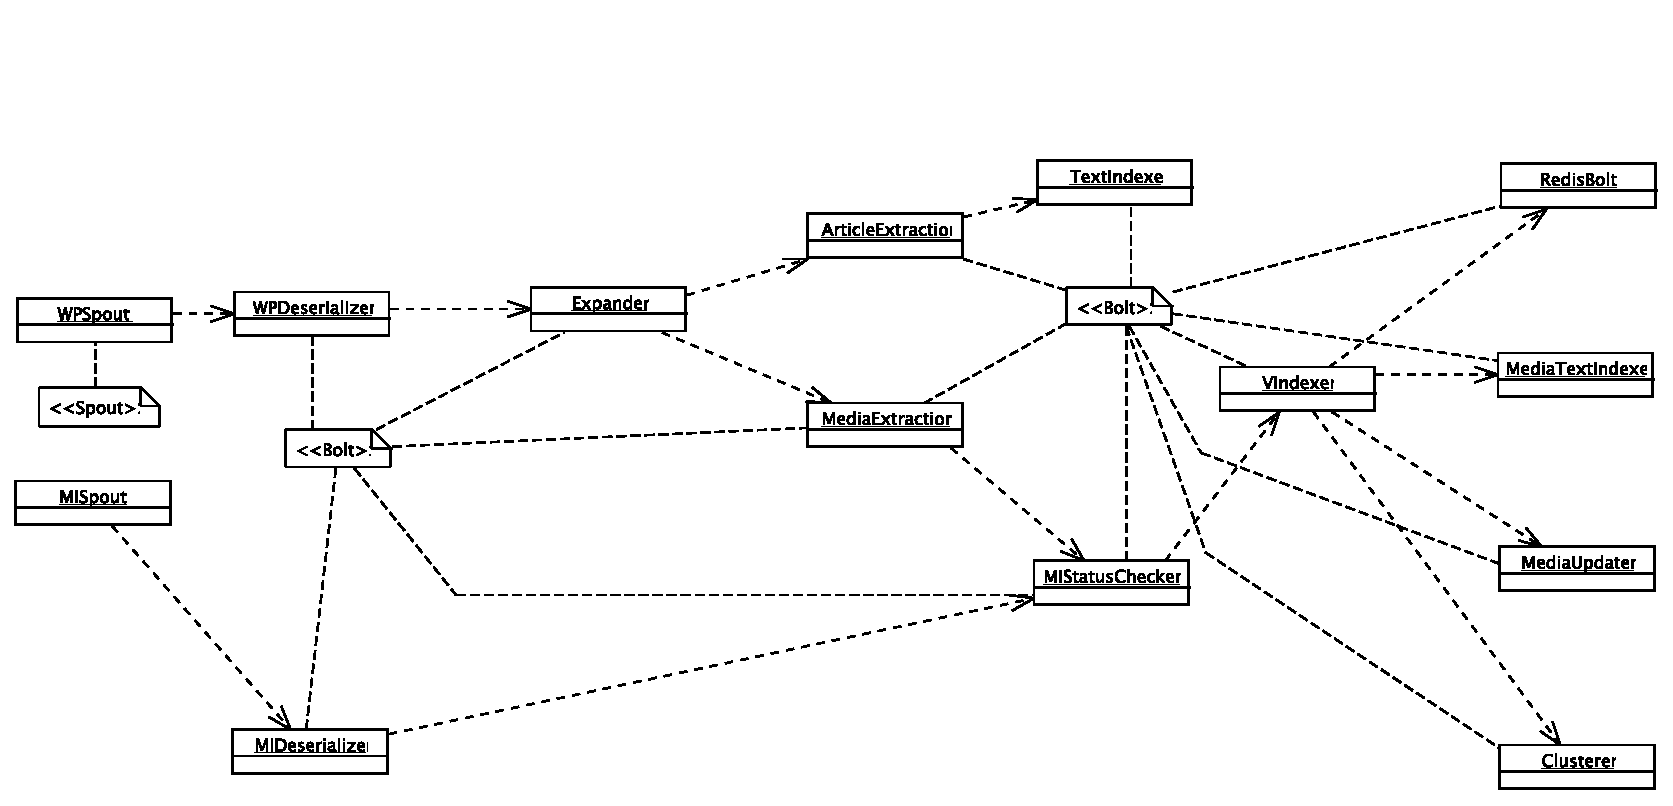
\includegraphics[width=12cm]{images/socialsensorother}
%  \caption{A sample Storm topology (readable from left to right) using an UML object diagram in the SocialSensor App, notes identify types for nodes (i.e., Bolts or Spouts).}
%  \label{socialsensor-topology}
%\end{figure*}

\subsection{Research Solution Evaluation}

OSTIA's evaluation is threefold. 

First, we evaluated our solution using an industrial case-study offered by one of the industrial partners in the DICE EU H2020 Project consortium~\cite{dice2020}.
%\footnote{\url{http://www.dice-h2020.eu/}}.  
The
partner in question uses open-source social-sensing software to elaborate a
subscription-based big-data application that: (a) aggregates news assets from
various sources (e.g., Twitter, Facebook, etc.) based on user-desired
specifications (e.g., topic, sentiment, etc.); (b) presents and allows the
manipulation of data. The application in question is based on the SocialSensor
App~\cite{socialsensor}
%\footnote{\url{https://github.com/socialsensor}} 
%(see
%Fig. \ref{socialsensor-topology} for a sample realised using a simple UML object diagram).  In particular, the topology in
%Fig. \ref{socialsensor-topology} extracts data from sources and divides and arranges contents based on type (e.g., article vs. media),
%later updating a series of databases (e.g., Redis) with these elaborations.

which features the combined
action of three complex streaming topologies based on Apache Storm. The
models that OSTIA elicited from this application were showcased to our
industrial partner in a focus group aimed at establishing the value of insights
produced as part of OSTIA-based analyses. Our qualitative assessment was based
on questionnaires and open discussion.

Second, to further confirm the validity of OSTIA analyses and support, we
applied it on two open-source applications featuring Big-Data analytics, namely: (a) the DigitalPebble application,
%\footnote{\url{https://github.com/DigitalPebble/storm-crawler}}, 
``A Text Classification API in Java originally developed by DigitalPebble Ltd. The
API is independent from the ML implementations used and can be used as a front
end to various ML algorithms" ~\cite{storm-crawler}; (b) the StormCV application, 
%\footnote{\url{https://github.com/sensorstorm/StormCV}} 
``StormCV
enables the use of Apache Storm for video processing by adding computer vision
(CV) specific operations and data model; the platform enables the development of
distributed video processing pipelines which can be deployed on Storm clusters" ~\cite{stormCV}.

%\begin{itemize}
%\item elaborate on the case-study partner
%\item elaborate on the case at hand for that partner
%\item elaborate on the origin of the application and how it uses social-sensor
%\item also, elaborate on the case by NETF which starts and stems from KILLRWEATHER
%\item should we elaborate on something else?
%\end{itemize}
%\textbf{TODO: @anyone, feel free to elaborate more!!}
Third, finally, as part of the OSTIA extension recapped in this manuscript, we applied formal verification approaches using the
Zot~\cite{zot}
%\footnote{\url{https://github.com/fm-polimi/zot}} 
LTL model-checker following an approach tailored from previous work \cite{icsoft,BRS15}.

%\comment{this section need a bit of refactoring it's not focused enough}
